% The underlying theory of the report

\subsection{One digital pixel}


Each pixel in the camera is constructed as shown in figure~\ref{fig:pixelschematic}.
The photo diodes detecting the actual light does, in many ways, act as a current source dependent on the light on it, when a picture is taken this
current is let through M1 and used to charge CS.
Before each picture is taken, M2 is opened to reset the voltage stored over CS.

It is important that M1 and M2 are not let on simultaneously for extended periods of time as this results in a short circuit from VDD to VSS thorugh PD1.
While the photo diode limits the current, this still might lead to excessive power usage and subsequent heating issues over time.


\begin{figure}[htbp]
  \centering
  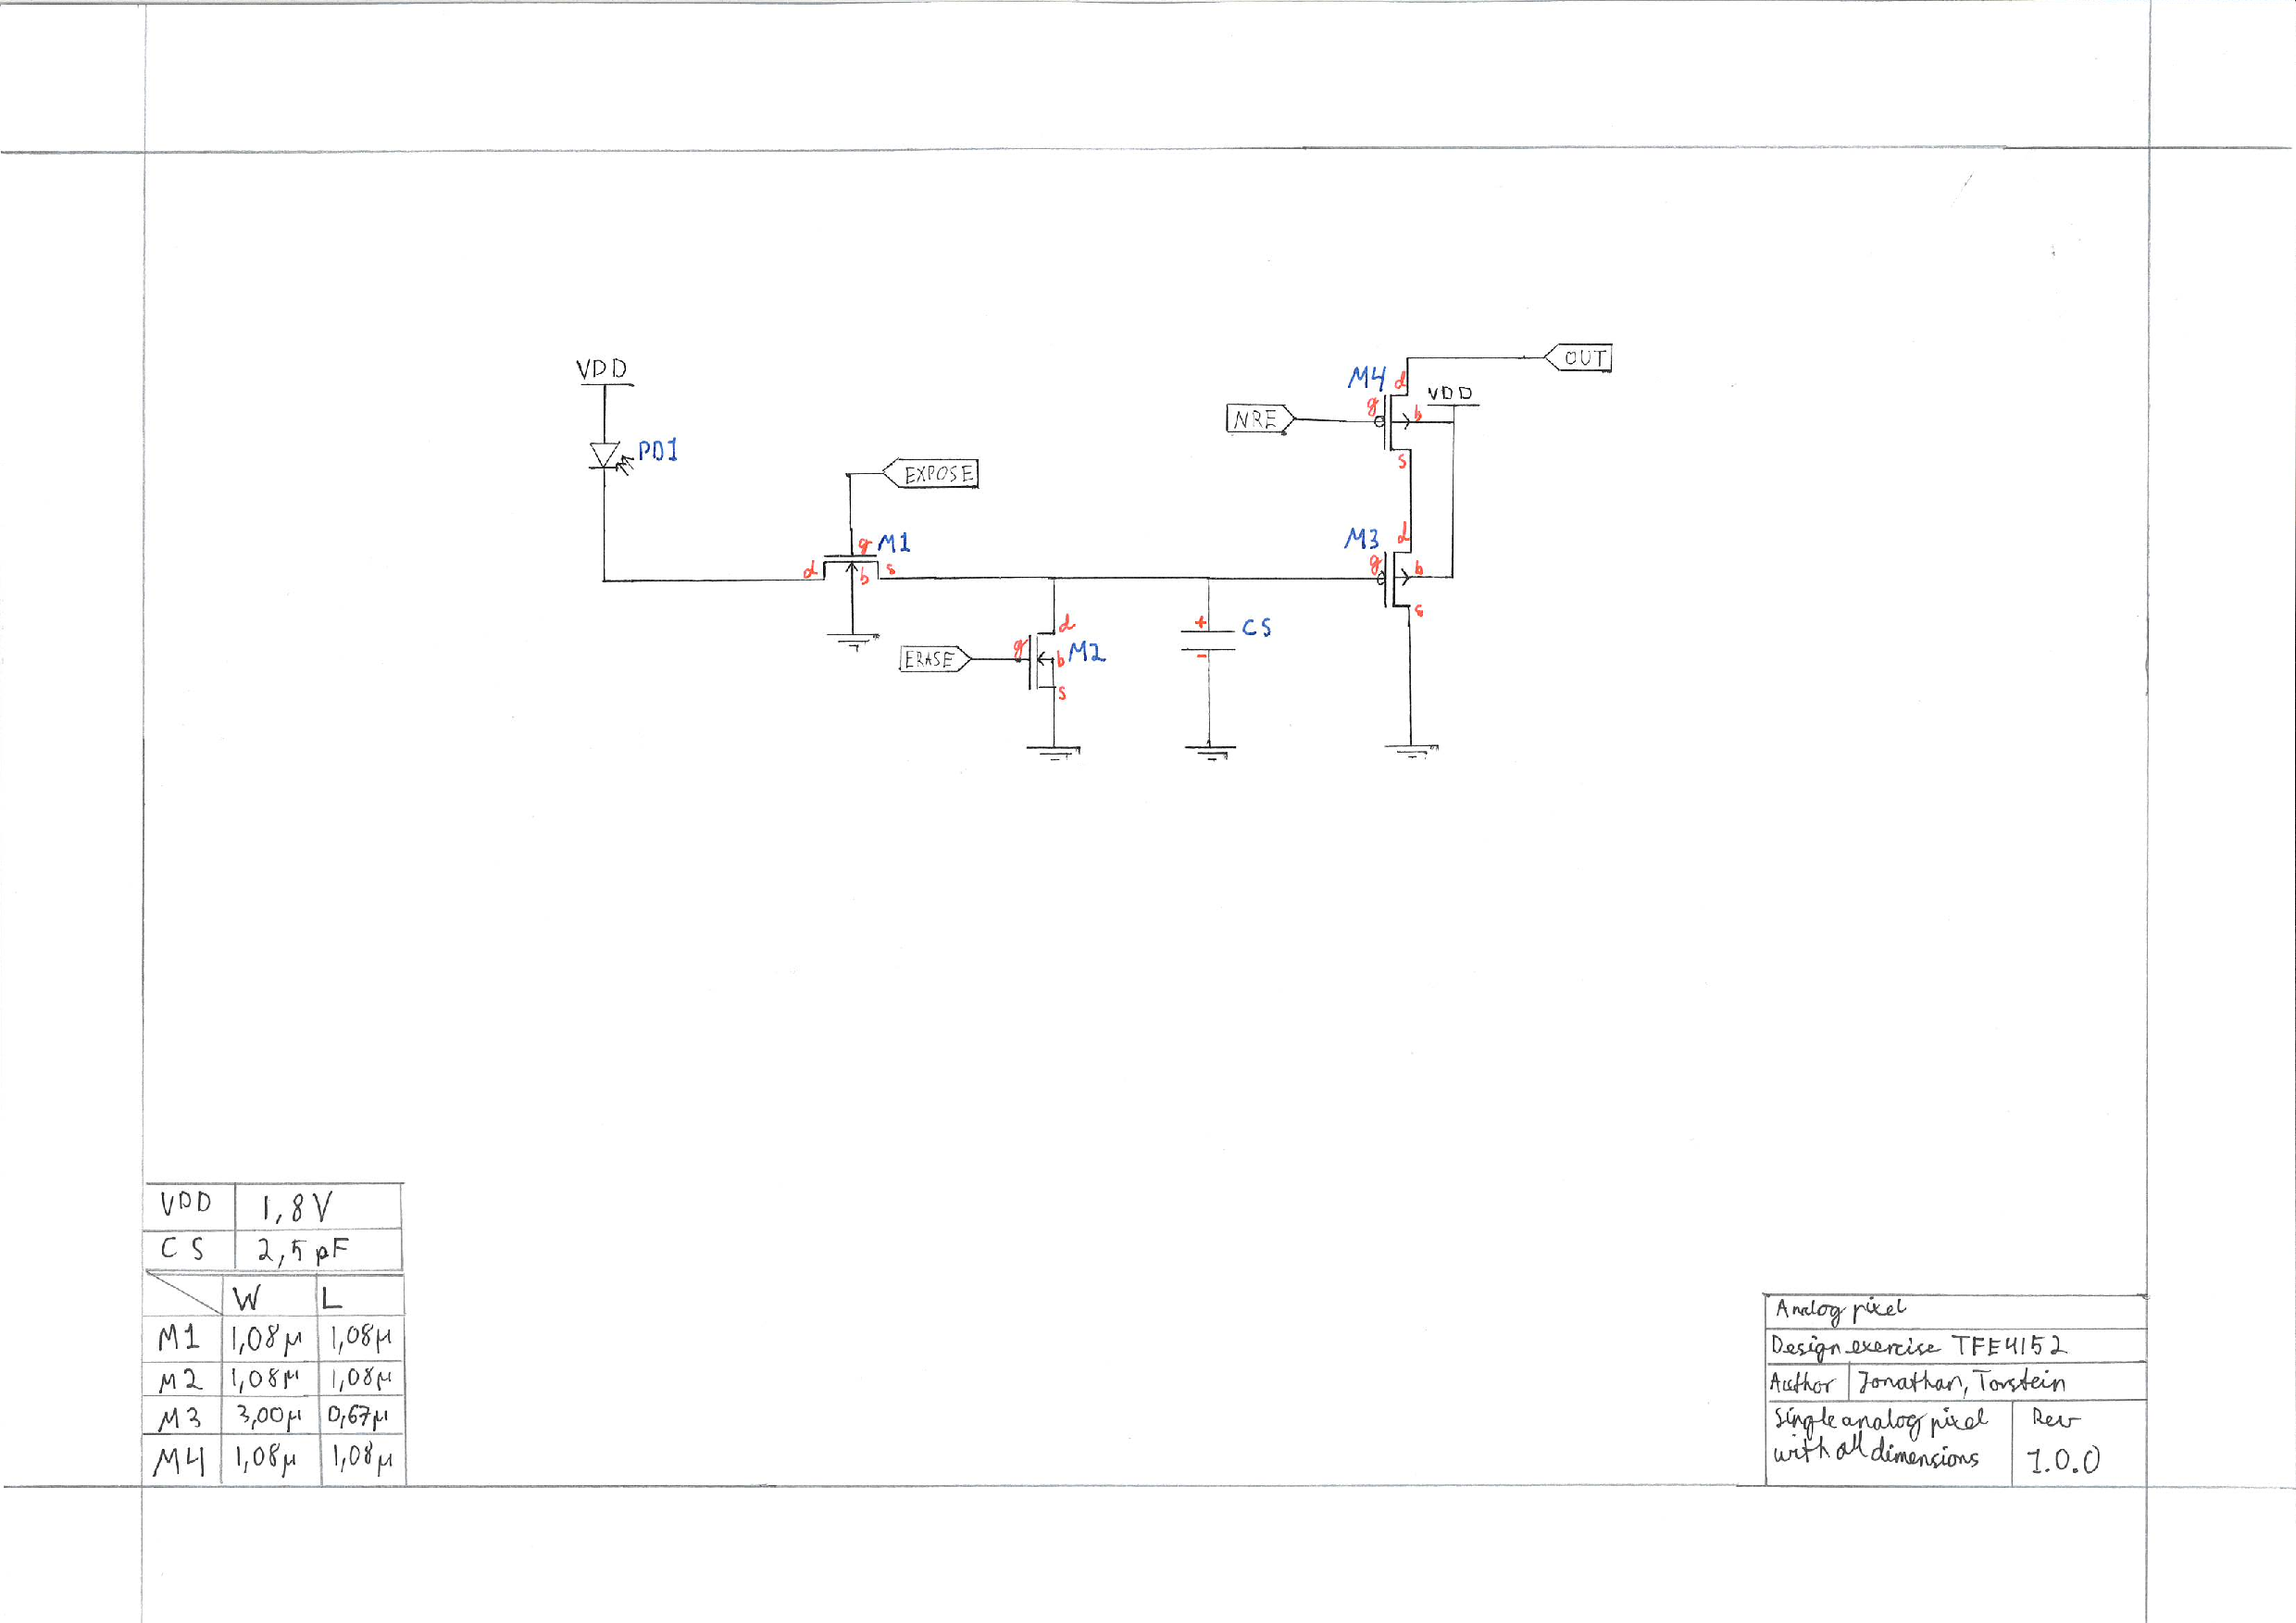
\includegraphics[width=0.85\textwidth]{figures/SchematicPixel}
  \caption{Schematic of one pixel with readout circuit, figure also exists bigger in Appendix~\ref{ap:Schematics}}
  \label{fig:pixelschematic}
\end{figure}


M3 is used to convert the voltage stored over CS into a variable resistance between N3 and VSS for a nondestructive readout of the pixel,
M4 functions as a simple switch to isolate the pixel from OUT to free the wire when other pixels in the camera are using it.



\subsection{Leakage through transistors}

As described in the analog book~\cite{AnalogBook} stuff can happen.

\subsection{Conceptual workings of a camera controller}

This might work...